\section{Dimensión territorial de la participación}

Las tablas externas aportan una geografía que los registros académicos no contienen. El SECOP registra el departamento de la entidad que contrata a cada graduado y el RUES asocia cada empresa a una cámara de comercio. Al cruzar esa geografía con la sede de origen del egresado, la huella territorial de la Universidad deja de ser una abstracción y se vuelve medible: revela dónde trabaja y se registra en el RUES quien estudió en cada sede, hasta qué punto la participación de los 174.685 graduados se arraiga en los territorios donde la institución mantiene presencia, y cómo la modalidad a distancia proyecta esa huella mucho más allá de las ciudades sede.

\subsection{Dónde contratan los graduados (SECOP)}
La contratación pública de los graduados se concentra en los departamentos donde la Universidad tiene sede. Bogotá D.C. encabeza con 137.117 contratos, seguida de Santander con 56.876 y Boyacá con 41.709. El Meta aporta 19.694 y Cundinamarca 16.858, de modo que los territorios líderes corresponden a las regiones de las sedes de Bogotá, Bucaramanga, Tunja y Villavicencio, junto con el área de influencia inmediata de la capital. Por debajo aparecen Casanare con 9.447 contratos y Antioquia con 8.810, este último vinculado a la presencia en Medellín, seguidos de departamentos de menor peso como Norte de Santander, Cesar, Tolima, Valle del Cauca y Huila (Figura~\ref{fig:secopdep}). La actividad contractual de los egresados no se dispersa de forma homogénea por el país, sino que gravita alrededor de los nodos donde la institución forma profesionales.

\begin{figure}[H]\centering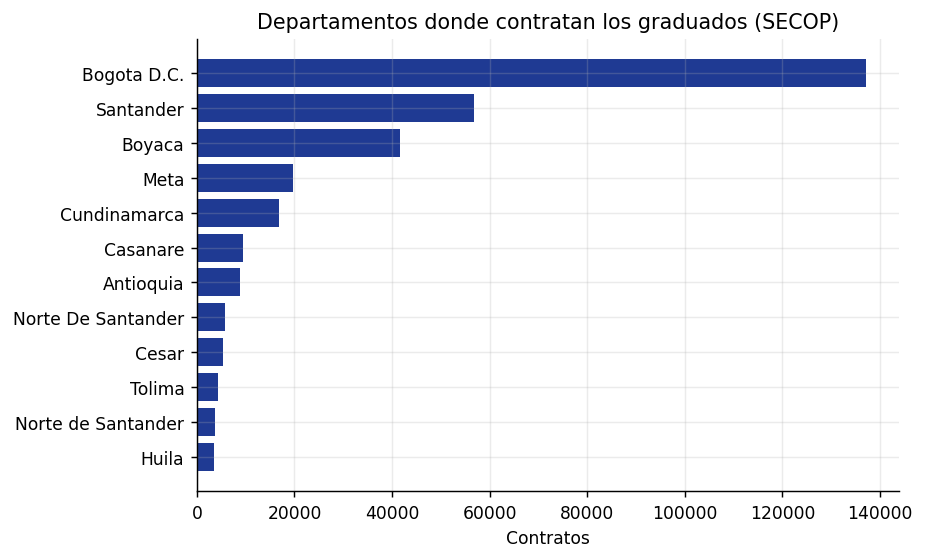
\includegraphics[width=0.78\linewidth]{figs_cruce/17_secop_departamento.png}
\caption{Departamentos de las entidades con las que contratan los graduados de la USTA (número de contratos, SECOP).}\label{fig:secopdep}\end{figure}

\subsection{Dónde registran empresa (RUES)}
La matrícula mercantil dibuja una geografía equivalente. La cámara de comercio de Bogotá registra 10.238 empresas de graduados, la de Bucaramanga 7.747, la de Tunja 3.326 y la de Villavicencio 2.516, todas correspondientes a ciudades sede de la Universidad. La cámara de Medellín para Antioquia suma 656 empresas, en línea con el tamaño de esa sede. Entre esas posiciones se intercalan cámaras del oriente y del piedemonte que prolongan el radio de influencia de las sedes ---Cúcuta con 1.151 empresas, Casanare con 821, Duitama con 815, Sogamoso con 642 y Barrancabermeja con 637, junto con Huila y Facatativá--- (Figura~\ref{fig:ruescam}). Tanto en la contratación pública como en la creación de empresas, los territorios de las sedes ocupan una y otra vez las primeras posiciones.

\begin{figure}[H]\centering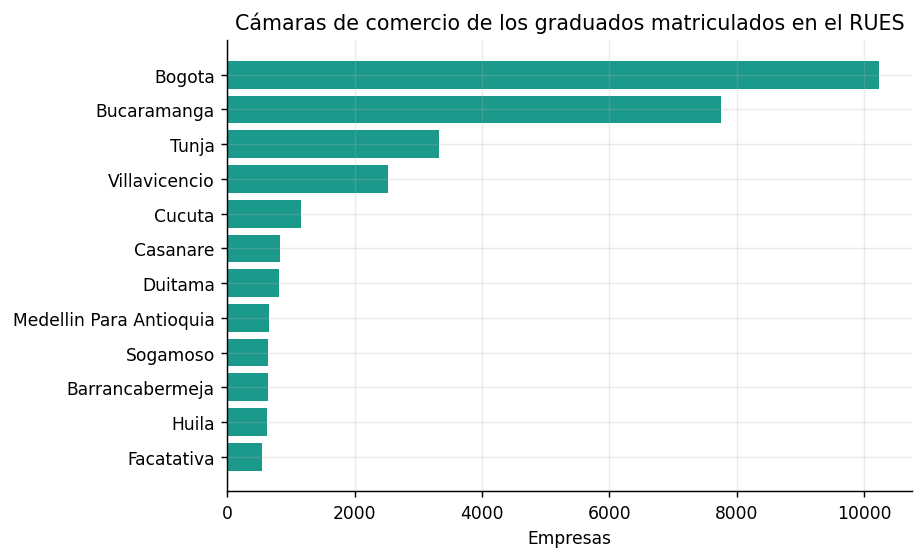
\includegraphics[width=0.78\linewidth]{figs_cruce/18_rues_camara.png}
\caption{Cámaras de comercio donde los graduados matriculados en el RUES registran sus empresas (RUES).}\label{fig:ruescam}\end{figure}

\subsection{Arraigo regional por sede}
Al descomponer la geografía por sede de origen, el arraigo se hace explícito: cada sede contrata y se registra en el RUES, sobre todo, dentro de su propio departamento. La Tabla~\ref{tab:arraigo} resume esa concentración y las Figuras~\ref{fig:secopreg} y~\ref{fig:ruesreg} la despliegan por completo. En la contratación pública, entre el 59\,\% y el 70\,\% de los contratos de cada sede se firma con entidades de su propio departamento; en la matrícula mercantil, la concentración es todavía mayor y culmina en Villavicencio, donde el 88,1\,\% de las empresas de sus graduados se registra en la cámara local, la cifra más alta de todo el sistema.

\begin{table}[H]
\centering
\caption{Concentración de la huella en el departamento de la sede de origen.}
\label{tab:arraigo}
\begin{tabularx}{0.93\linewidth}{Xlrr}
\toprule
\rowcolor{ustaazul}\textbf{\color{white}Sede} & \textbf{\color{white}Departamento} & \textbf{\color{white}Contratos en su depto.} & \textbf{\color{white}Empresas en su cámara} \\
\midrule
Bogotá & Bogotá D.C. & 61,8\,\% & 48,8\,\% \\
Bucaramanga & Santander & 59,6\,\% & 63,4\,\% \\
Tunja & Boyacá & 59,2\,\% & 60,7\,\% \\
Villavicencio & Meta & 66,7\,\% & 88,1\,\% \\
Medellín & Antioquia & 69,6\,\% & --- \\
\bottomrule
\end{tabularx}
\end{table}

\begin{figure}[H]\centering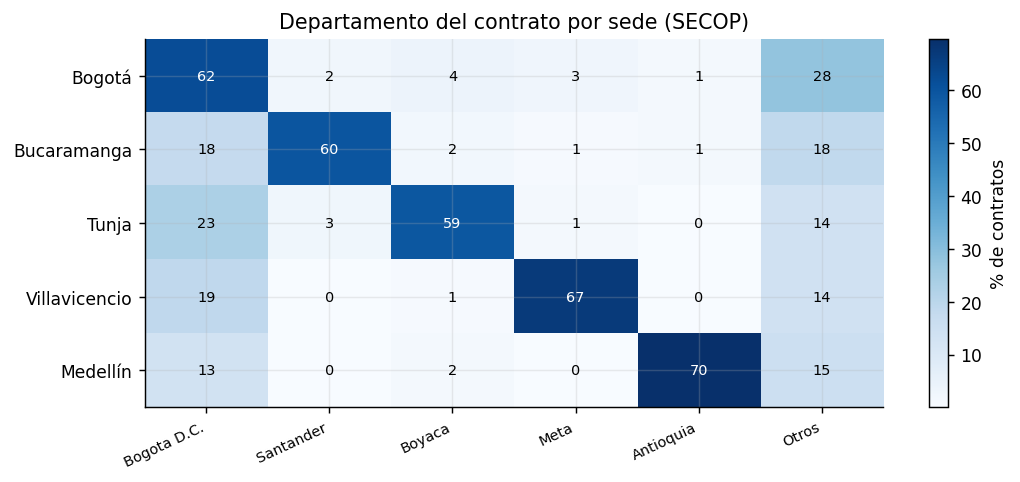
\includegraphics[width=0.85\linewidth]{figs_cruce/19_secop_seccional_region.png}
\caption{Distribución del departamento de contratación según la sede de origen del graduado (\% de contratos por fila, SECOP).}\label{fig:secopreg}\end{figure}

\begin{figure}[H]\centering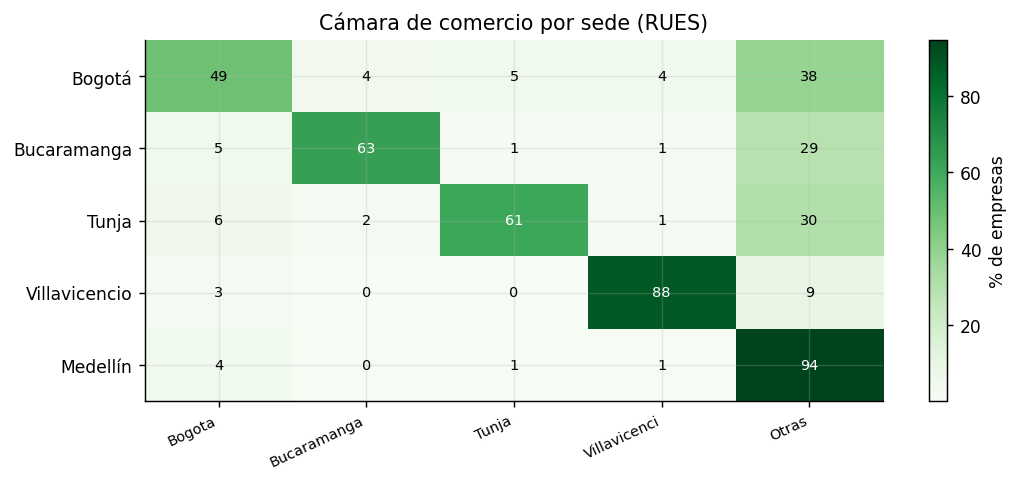
\includegraphics[width=0.85\linewidth]{figs_cruce/20_rues_seccional_camara.png}
\caption{Distribución de la cámara de comercio de registro según la sede de origen del graduado (\% de empresas por fila, RUES).}\label{fig:ruesreg}\end{figure}

Por encima de ese predominio regional, la capital opera como un segundo polo de atracción para todas las sedes. Tras su propio departamento, los graduados de Tunja dirigen el 23,1\,\% de sus contratos a entidades de Bogotá D.C., los de Bucaramanga el 17,7\,\%, los de Villavicencio el 18,7\,\% y los de Medellín el 13,4\,\%. Esa atracción no desplaza el arraigo local, pero refleja la gravitación natural de las entidades del orden nacional, concentradas en la capital, sobre los contratistas de todo el país. El mapa que resulta es de doble nivel: una base sólida de participación regional sobre la que se monta un vínculo secundario y común con el centro administrativo de la Nación.

\subsection{La huella nacional de la educación a distancia}
El patrón de arraigo regional encuentra su excepción ---y su complemento--- en la modalidad a distancia. Los graduados de los centros VUAD, que la Universidad sostiene en decenas de municipios sin campus presencial, no se concentran en un único departamento, sino que riegan su huella por todo el país. Sus contratos se reparten entre Bogotá D.C. (2.916), Boyacá (1.489), Casanare (1.179), Santander (1.065) y, de manera reveladora, departamentos donde la institución no tiene sede física, como Nariño (967), Quindío (956), el Meta (869) y Cundinamarca (710). Mientras las sedes presenciales irradian participación sobre su entorno inmediato, la educación a distancia proyecta la presencia de la Universidad sobre la geografía nacional, alcanzando regiones que de otro modo quedarían fuera de su radio. La huella territorial del egresado tomasino tiene, así, dos formas complementarias: la concentrada de las sedes presenciales y la difusa de la modalidad a distancia.

\begin{cajahallazgo}
La participación del egresado es profundamente regional. Lejos de dispersarse por todo el país, la contratación pública y la matrícula mercantil de los graduados se concentran en el departamento de su sede de origen, en proporciones que van del 59\,\% al 70\,\% en el SECOP y hasta el 88\,\% en el RUES, con Bogotá como único destino nacional compartido. Cada sede nutre de forma directa el tejido productivo e institucional de su territorio, de modo que la presencia de la Universidad en seis sedes se traduce en otros tantos polos de desarrollo regional, mientras la modalidad a distancia extiende esa huella a departamentos sin campus propio. La institución no solo forma profesionales, sino que actúa como motor del desarrollo de las regiones donde se asienta, retornando a cada territorio el talento que en él se ha formado.
\end{cajahallazgo}
